\documentclass{jhwhw}

\linespread{1.2}

\usepackage[T1]{fontenc}\usepackage{palatino}
\usepackage{amssymb,amsmath,amsthm,mathtools}
\usepackage[english]{babel}
\usepackage[utf8]{inputenc}
\usepackage[babel]{csquotes}
\usepackage[pdftex]{hyperref}
\usepackage{enumitem}

\usepackage{graphicx} 
\usepackage{verbatim} % Commenti in blocco con \begin{comment}
\usepackage{bm}
\usepackage[font={small,it}]{caption}
\usepackage{subcaption}
\usepackage{geometry}
\usepackage{array}
\usepackage{enumitem}
\setlist[enumerate]{label*=\arabic*.}
	
\usepackage{algorithm}
\usepackage[noend]{algpseudocode}

\makeatletter
\def\BState{\State\hskip-\ALG@thistlm}
\makeatother

% Simbolo iid
\newcommand\iid{\stackrel{\mathclap{\normalfont\tiny\mbox{iid}}}{\sim}}
% Simbolo ind
\newcommand\ind{\stackrel{\mathclap{\normalfont\tiny\mbox{ind}}}{\sim}}

\title{SDS 385: Homework 1}
\author{G.~Paulon}

\begin{document}

\problem{Linear regression}

\begin{enumerate}[label=(\Alph*)]
\item Let us write the WLS objective (or cost) function $$l (\beta) = \sum_{i=1}^N \frac{w_i}{2} (y_i - x_i^T \beta)^2$$ in a matricial form. We get 
\begin{align*}
l(\beta) &= \frac{1}{2} (y - X \beta)^T W (y - X \beta)
\\
&= \frac{1}{2} (y^T - (X \beta)^T) W (y - X \beta)
\\
&= \frac{1}{2} \left( y^T W y - y^T W X \beta - (X \beta)^T W y + (X \beta)^T W X \beta \right) 
\end{align*}
Let us remark here that the second and the third term of the sum can be collected in one single term. In fact 
$$(y^T W X \beta)^T = (X \beta)^T W y,$$ i.e. the first is the transposed of the second but, since they are real numbers, they are also equal. Hence we have
\begin{equation*}
l(\beta) = \frac{1}{2} \left( y^T W y - 2 \beta^T X^T W y + \beta^T X^T W X \beta \right). 
\end{equation*}

We now use the second-order sufficient condition to find the local optimum. To do this, we first need to calculate the gradient of the WLS objective function equalizing it to $0$. Thus, 
\begin{align*}
&\nabla l (\hat{\beta}) = 0
\\
\Leftrightarrow &\frac{1}{2} (- 2 X^T W y + 2 X^T W X \hat{\beta}) = 0
\\
\Leftrightarrow &(X^T W X) \hat{\beta} = X^T W y,
\end{align*}
which is the set of desired equations (also known as normal equations). 

The second order condition for a minimum requires that the hessian of the objective function, i.e. the matrix $X^T W X$ is positive definite. This requirement is fulfilled and it is easy to verify in case $X$ has full rank (i.e. the columns of $X$ are linearly independent).

\item Since the matrix $X^T W X$ is definite positive, it is also nonsingular and therefore its inverse matrix exists. The normal equation can be easily solved by inverting the matrices, which leads to
$$\hat{\beta} = (X^T W X)^{-1} X^T W y.$$
The classical inversion method, however, is not recommended as its computational complexity grows rapidly as the dimension of the matrices increases. Moreover, the inversion of a matrix is not stable numerically speaking, as for some matrices the numerical solution does not approach the exact one.

For these reasons, we present here two other approaches that are used to deal with the solution of linear systems: the LU and the Cholesky factorizations. 
\begin{itemize}
\item The LU factorization consists in finding two matrices $L$ (lower triangular) and $U$ (upper triangular) such that the matrix $A$ of the system of equations $Ax = b$ can be written as their product. Therefore we get $LUx = b$, which can be solved sequentially by two simple systems
\begin{align*}
&Lq = b
\\
&Ux = q
\end{align*}
In our case, the pseudocode can be summarized as follows.
\begin{algorithm}
\caption{LU solver}\label{alg:lu}
\begin{algorithmic}[1]
\Procedure{My\_LU}{X, y, W}
\State find the factors $L, U$, s.t. $X^TWX = LU$
\State solve the first linear system: $q \gets L^{-1} X^TWy$
\State solve the second linear system: $\hat{\beta} \gets U^{-1} q$
\EndProcedure
\end{algorithmic}
\end{algorithm}

\item The Cholesky factorization can be found for symmetric and positive definite matrices, and it consists in factorizing the original matrix as $A = RR^T$, where $R$ is a lower triangular matrix. 

In our case, the pseudocode can be summarized as follows.
\begin{algorithm}
\caption{Cholesky solver}\label{alg:chol}
\begin{algorithmic}[1]
\Procedure{My\_Chol}{X, y, W}
\State find the factor $R$, s.t. $X^TWX = RR^T$
\State solve the first linear system: $q \gets R^{-1} X^TWy$
\State solve the second linear system: $\hat{\beta} \gets R^{-T} q$
\EndProcedure
\end{algorithmic}
\end{algorithm}
\end{itemize}

\item We here compare the three methods used to solve the linear system of the normal equations. Let us point out that in each of the three algorithms we exploited the fact that $W$ is a diagonal matrix, optimizing the matricial product $X^TW$ by simply multiplying the first element of the diagonal of $W$ by the first column of $X^T$, and so on.

The performances of the three algorithms are displayed in Figure \ref{fig:perf1}. Four test cases were analysed: the values of $N$ and $P$ range from a minimum of $(N,P) = (500,50)$ to a maximum of $(N,P) = (5000,2000)$. As one can see, both the Cholesky factorization and the LU method largely outperform the inversion method. This is more evident for high dimensional datasets, when the inversion of the design is hard to compute.

\begin{figure}[!ht]
\centering
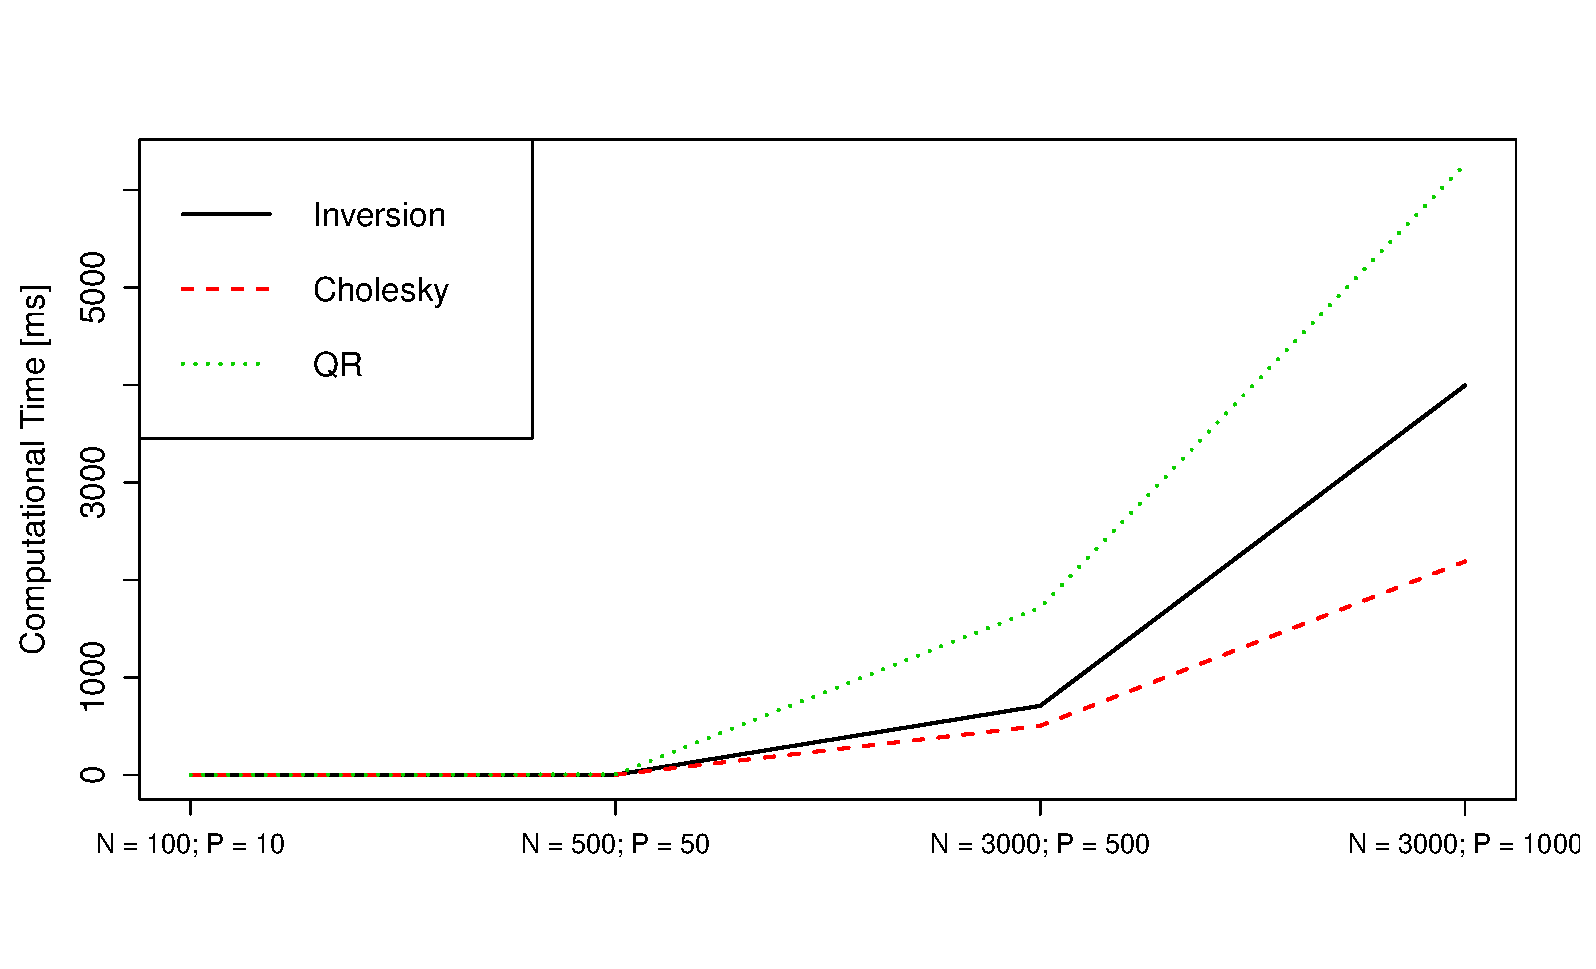
\includegraphics[width=0.6\columnwidth]{./Img/perf}
\caption{Comparison between the performances of the three algorithms for different dimensions of the data and of their features.}
\label{fig:perf1}
\end{figure}

\item Now, if $X$ is a highly sparse matrix, one can exploit appropriate routines in R language in order to make the computation faster. 

\begin{figure}[!ht]
\centering
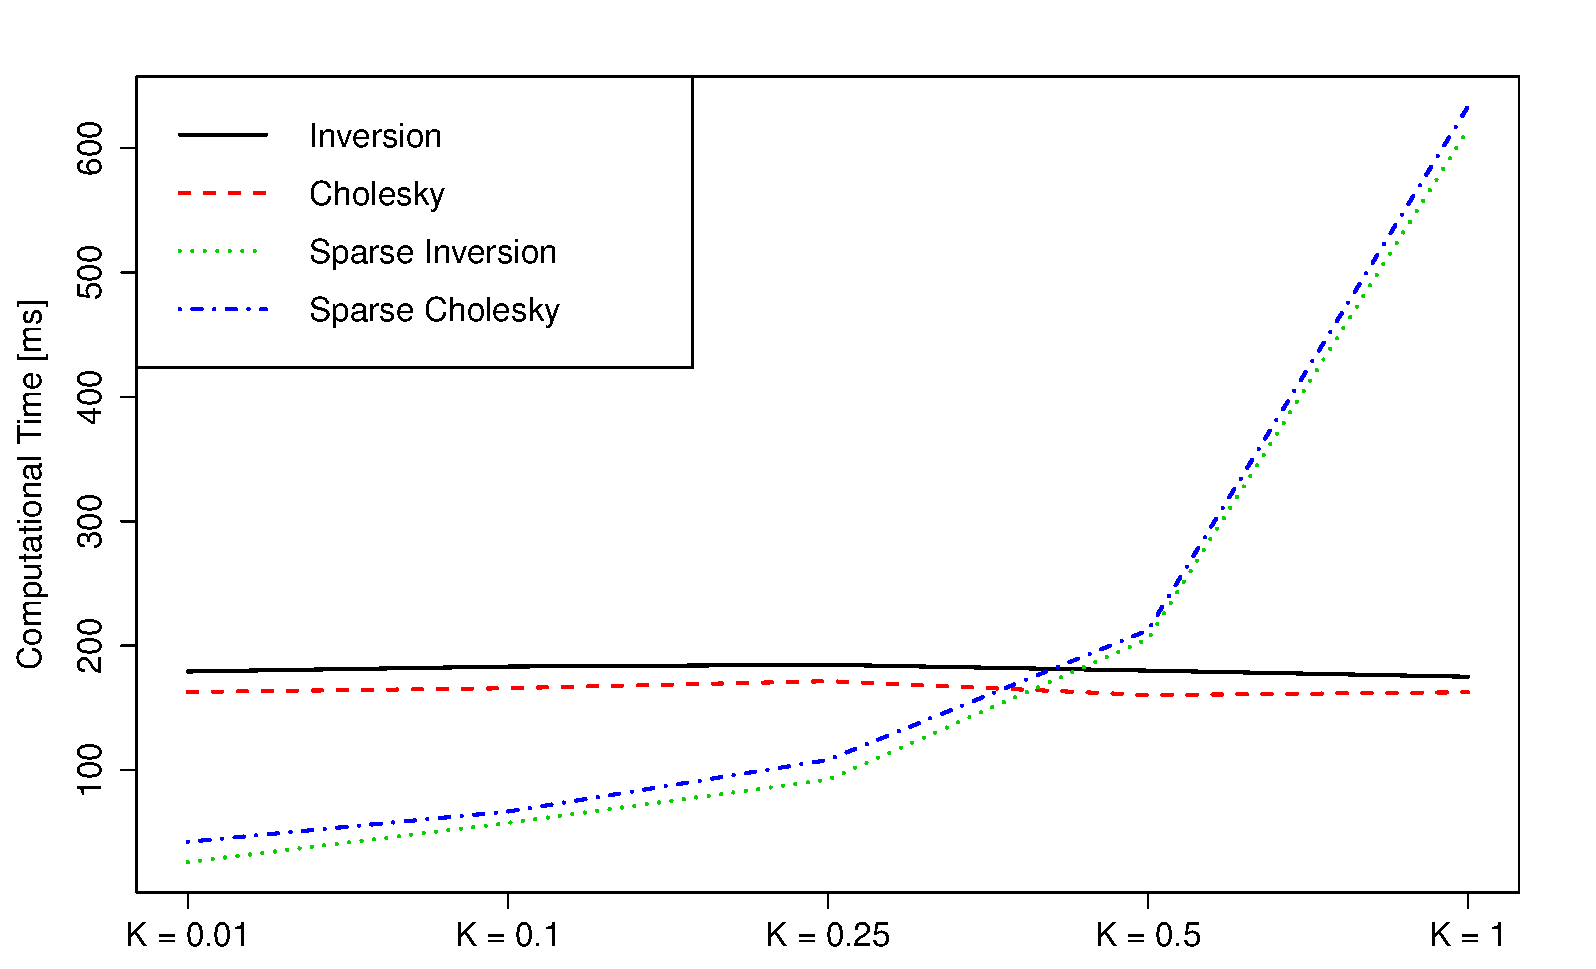
\includegraphics[width=0.6\columnwidth]{./Img/perf_2}
\caption{Comparison between the performances of the three algorithms for different sparsity levels $K$.}
\label{fig:perf2}
\end{figure}

Let us take, as an example, $(N, P) = (2500,1000)$ and let us compare the results for different levels of sparsity $K$ of the matrix $X$. As one can see in Figure \ref{fig:perf2}, when the features matrix is dense, the previous methods outperform the sparse method, as this latter involves a first stage in which $X$ is converted in a sparse format. However, as $K$ increases, the sparse method becomes significantly faster than the others. This is due to the fact that matricial products are more efficient in a sparse format and a lot of useless computations is avoided.

\end{enumerate}

\problem{Generalized linear models}

\begin{enumerate}[label=(\Alph*)]
\item The negative log-likelihood for the problem of logistic regression can be written as
\begin{align*}
l(\beta) &= - \log\left\lbrace \prod_{i=1}^N p(y_i | \beta) \right\rbrace
\\
&= -\sum_{i=1}^N \left\lbrace \log \binom{m_i}{y_i} + y_i \log(w_i) + (m_i - y_i) \log (1 - w_i) \right\rbrace.
\end{align*}
The gradient of this latter expression is 
\begin{align*}
\nabla l(\beta) &= - \sum_{i=1}^N \left\lbrace y_i \frac{1}{w_i} \frac{x_i e^{-x_i^T \beta}}{(1+e^{-x_i^T \beta})^2} - (m_i - y_i) \frac{1}{1-w_i} \frac{x_i e^{-x_i^T \beta}}{(1+e^{-x_i^T \beta})^2} \right\rbrace
\\
&= - \sum_{i=1}^N \left\lbrace y_i \frac{x_i e^{-x_i^T \beta}}{1+e^{-x_i^T \beta}} - m_i \frac{x_i}{1+e^{-x_i^T \beta}} + y_i \frac{x_i}{1+e^{-x_i^T \beta}} \right\rbrace
\\
&= - \sum_{i=1}^N \left\lbrace y_i x_i - m_i \frac{x_i}{1+e^{-x_i^T \beta}} \right\rbrace
\\
&= - \sum_{i=1}^N \left\lbrace x_i (y_i - m_i w_i) \right\rbrace
\\
&= -X^T (y - mw).
\end{align*}

\item

\item In order to write the second-order Taylor approximation, we first need to compute the Hessian of the negative log-likelihood, that is
\begin{align*}
\nabla^2 l(\beta) &= \nabla \left( - \sum_{i=1}^N x_i (y_i - m_i w_i) \right)
\\
&= \left( \sum_{i=1}^N \nabla (m_i x_{i1} w_i); \dots ; \sum_{i=1}^N \nabla (m_i x_{ip} w_i) \right).
\end{align*}

By exploiting the fact that $\frac{\partial w_i}{\partial \beta_j} = x_{ij} w_i (1 - w_i)$, we obtain, 
\begin{align*}
\nabla^2 l(\beta) &= \left( \begin{array}{ccc}
\sum_{i=1}^N m_i x_{i1} x_{i1} w_i (1 - w_i) & \hdots & \sum_{i=1}^N m_i x_{ip} x_{i1} w_i (1 - w_i) \\ 
\vdots & \ddots & \vdots \\ 
\sum_{i=1}^N m_i x_{i1} x_{ip} w_i (1 - w_i) & \hdots & \sum_{i=1}^N m_i x_{ip} x_{ip} w_i (1 - w_i)
\end{array} 
\right)
\\
&= X^T W X, 
\end{align*}
where the matrix W is defined as $W = \text{diag} \{ m_1 w_1 (1-w_1); \dots ; m_N w_N (1-w_N) \}$. 

The second order Taylor expansion is then 
\begin{align*}
\tilde{l} (\beta) &= l (\beta_0) + \nabla l (\beta_0)^T (\beta - \beta_0) + \frac{1}{2} (\beta - \beta_0)^T \nabla^2 l (\beta_0) (\beta - \beta_0)
\\
&= l (\beta_0) - (y - m w)^T X (\beta - \beta_0) + \frac{1}{2} (\beta - \beta_0)^T X^T W X (\beta - \beta_0)
\\
&= l (\beta_0) - (y-mw)^T X \beta + (y - mw)^T X \beta_0 
\\
&\quad + \frac{1}{2} \beta^T X^T W X \beta + \frac{1}{2} \beta_0^T X^T W X \beta_0 - \beta_0^T X^T W X \beta
\\
&=l (\beta_0) + (y - mw)^T X \beta_0 + \frac{1}{2} \beta_0^T X^T W X \beta_0 
\\
&\quad - (y - mw + WX\beta_0)^T X \beta + \frac{1}{2} (X \beta)^T W (X \beta)
\\
&=\frac{1}{2} ( z - X \beta)^T W ( z - X \beta) + c,
\end{align*}
where 
\begin{align*}
&z = -W^{-1} (y - mw + WX \beta_0) = W^{-1}(mw - y) - X \beta_0;
\\
&c = l(\beta_0) + (y - mw)^T X \beta_0 + \frac{1}{2} \beta_0^T X^T W X \beta_0 
\\
&\quad \text{ } - \frac{1}{2} (y - mw + WX \beta_0)^T W^{-1} (y - mw + WX \beta_0).
\end{align*}


\end{enumerate}


\end{document}
